\documentclass{article}
\usepackage{minted}
\usepackage{listings}
\usepackage{graphicx}
\usepackage{physics}
\usepackage{siunitx}
\usepackage{placeins}
\usepackage{hyperref}

\usepackage{lmodern}
\usepackage{amssymb,amsmath}
\usepackage{ifxetex,ifluatex}
\usepackage{fixltx2e} % provides \textsubscript
\ifnum 0\ifxetex 1\fi\ifluatex 1\fi=0 % if pdftex
  \usepackage[T1]{fontenc}
  \usepackage[utf8]{inputenc}
  \usepackage{textcomp} % provides euro and other symbols
\else % if luatex or xelatex
  \usepackage{unicode-math}
  \defaultfontfeatures{Ligatures=TeX,Scale=MatchLowercase}
\fi
% use upquote if available, for straight quotes in verbatim environments
\IfFileExists{upquote.sty}{\usepackage{upquote}}{}
% use microtype if available
\IfFileExists{microtype.sty}{%
\usepackage[]{microtype}
\UseMicrotypeSet[protrusion]{basicmath} % disable protrusion for tt fonts
}{}
\IfFileExists{parskip.sty}{%
\usepackage{parskip}
}{% else
\setlength{\parindent}{0pt}
\setlength{\parskip}{6pt plus 2pt minus 1pt}
}
\usepackage{hyperref}
\hypersetup{
            pdfborder={0 0 0},
            breaklinks=true}
\urlstyle{same}  % don't use monospace font for urls
\usepackage{color}
\usepackage{fancyvrb}
\newcommand{\VerbBar}{|}
\newcommand{\VERB}{\Verb[commandchars=\\\{\}]}
\DefineVerbatimEnvironment{Highlighting}{Verbatim}{commandchars=\\\{\}}
% Add ',fontsize=\small' for more characters per line
\newenvironment{Shaded}{}{}
\newcommand{\AlertTok}[1]{\textcolor[rgb]{1.00,0.00,0.00}{\textbf{#1}}}
\newcommand{\AnnotationTok}[1]{\textcolor[rgb]{0.38,0.63,0.69}{\textbf{\textit{#1}}}}
\newcommand{\AttributeTok}[1]{\textcolor[rgb]{0.49,0.56,0.16}{#1}}
\newcommand{\BaseNTok}[1]{\textcolor[rgb]{0.25,0.63,0.44}{#1}}
\newcommand{\BuiltInTok}[1]{#1}
\newcommand{\CharTok}[1]{\textcolor[rgb]{0.25,0.44,0.63}{#1}}
\newcommand{\CommentTok}[1]{\textcolor[rgb]{0.38,0.63,0.69}{\textit{#1}}}
\newcommand{\CommentVarTok}[1]{\textcolor[rgb]{0.38,0.63,0.69}{\textbf{\textit{#1}}}}
\newcommand{\ConstantTok}[1]{\textcolor[rgb]{0.53,0.00,0.00}{#1}}
\newcommand{\ControlFlowTok}[1]{\textcolor[rgb]{0.00,0.44,0.13}{\textbf{#1}}}
\newcommand{\DataTypeTok}[1]{\textcolor[rgb]{0.56,0.13,0.00}{#1}}
\newcommand{\DecValTok}[1]{\textcolor[rgb]{0.25,0.63,0.44}{#1}}
\newcommand{\DocumentationTok}[1]{\textcolor[rgb]{0.73,0.13,0.13}{\textit{#1}}}
\newcommand{\ErrorTok}[1]{\textcolor[rgb]{1.00,0.00,0.00}{\textbf{#1}}}
\newcommand{\ExtensionTok}[1]{#1}
\newcommand{\FloatTok}[1]{\textcolor[rgb]{0.25,0.63,0.44}{#1}}
\newcommand{\FunctionTok}[1]{\textcolor[rgb]{0.02,0.16,0.49}{#1}}
\newcommand{\ImportTok}[1]{#1}
\newcommand{\InformationTok}[1]{\textcolor[rgb]{0.38,0.63,0.69}{\textbf{\textit{#1}}}}
\newcommand{\KeywordTok}[1]{\textcolor[rgb]{0.00,0.44,0.13}{\textbf{#1}}}
\newcommand{\NormalTok}[1]{#1}
\newcommand{\OperatorTok}[1]{\textcolor[rgb]{0.40,0.40,0.40}{#1}}
\newcommand{\OtherTok}[1]{\textcolor[rgb]{0.00,0.44,0.13}{#1}}
\newcommand{\PreprocessorTok}[1]{\textcolor[rgb]{0.74,0.48,0.00}{#1}}
\newcommand{\RegionMarkerTok}[1]{#1}
\newcommand{\SpecialCharTok}[1]{\textcolor[rgb]{0.25,0.44,0.63}{#1}}
\newcommand{\SpecialStringTok}[1]{\textcolor[rgb]{0.73,0.40,0.53}{#1}}
\newcommand{\StringTok}[1]{\textcolor[rgb]{0.25,0.44,0.63}{#1}}
\newcommand{\VariableTok}[1]{\textcolor[rgb]{0.10,0.09,0.49}{#1}}
\newcommand{\VerbatimStringTok}[1]{\textcolor[rgb]{0.25,0.44,0.63}{#1}}
\newcommand{\WarningTok}[1]{\textcolor[rgb]{0.38,0.63,0.69}{\textbf{\textit{#1}}}}
\setlength{\emergencystretch}{3em}  % prevent overfull lines
\providecommand{\tightlist}{%
  \setlength{\itemsep}{0pt}\setlength{\parskip}{0pt}}
\setcounter{secnumdepth}{0}
% Redefines (sub)paragraphs to behave more like sections
\ifx\paragraph\undefined\else
\let\oldparagraph\paragraph
\renewcommand{\paragraph}[1]{\oldparagraph{#1}\mbox{}}
\fi
\ifx\subparagraph\undefined\else
\let\oldsubparagraph\subparagraph
\renewcommand{\subparagraph}[1]{\oldsubparagraph{#1}\mbox{}}
\fi

% set default figure placement to htbp
\makeatletter
\def\fps@figure{htbp}
\makeatother

\graphicspath{{../figures/}}

\title{AMATH 582 Homework 3: PCA}
\author{Brady Griffith}

\begin{document}
    \maketitle

    \begin{abstract}
        A mass on a spring is recorded with 3 cameras each at different views.
        This problem has a known physical behavior, so it's an excellent candidate
        to preform PCA on and compare the results. Four cases are considered:
        purely vertical motion, the same with camera shake, vertical and
        horizontal motion, and vertical and horizontal motion with rotation of
        the mass. The spring mass motion and pendulum motion are all identifiable
        in the principle components in the cases without camera shake and rotation.
        The camera renders the image almost completely useless while the rotation
        just mixes the modes.
    \end{abstract}

    \section{Introduction and Overview}
    My undergraduate degree was in physics, so I have a particular fondness for
    the spring mass oscillator. This project takes a backwards look, as if the
    problem were novel physics to explain. Using videos taken at three different
    perspectives, I use principal component analysis to infer the physics of the
    mass/spring system. This particular problem has the advantage of a
    theoretical solution to compare results against.

    In the simplest version of this problem, the spring is constrained to only
    move vertically, i.e. without pendulum motion. This is the problem
    solved in the first week of any mechanics class, and for the mass's vertical
    displacement from equilibrium $z(t)$,
    \begin{equation}
        z(t) = z_0 \sin(\omega_Z t - \phi_0)
    \end{equation}
    where $z_0$ and $\phi_0$ are the initial displacement and phase, and
    $\omega_Z^2 = \frac{k}{m}$ is defined as the resonant frequency for the
    spring constant $k$ and mass $m$. When behaving in this limit, you would
    expect principal mode to be a sinusoid with that frequency.

    A more complicated version of this problem displaces the mass laterally as
    well, inducing a pendulum motion. The exact dynamics of this system are 
    complicated with precession of the pendulum motion and can involve coupling
    between modes \cite{Lynch2002}. Exact motion is not important to this
    analysis and only short time scales are considered. As long as the
    frequencies stay away from being in resonance, the two can be treated
    separately. We would then expect second and third modes asscociated with the
    elliptical pendulum motion.

    A similar problem is the example used in the textbook when explaining PCA
    \cite{Kutz2013}. The difference here being that instead of each perspective
    reporting a pendulum position, this projects looks at the unprocessed
    camera data. This probably isn't the best way to extract information about
    the motion, but does serve as a better exploration of PCA's limitations.

    \section{Theoretical Background}
    Principal component analysis in use for time series, as is the case in this
    problem, begins by collecting a vectors of each measurement's time series,
    $\vb*{x_i}$, into rows of a single large matrix.
    \begin{equation}
        \vb{X} = 
        \begin{bmatrix}
            \vb*{x_0}\\
            \vb*{x_1}\\
            \vdots \\
            \vb*{x_n}
        \end{bmatrix}
    \end{equation}

    The covariance of between all measurements is given by the matrix elements of
    \begin{equation}
        \vb{C}_{\vb{X}} = \frac{1}{n-1} \vb{X} \vb{X}^T
    \end{equation}
    It would be informative to switch into a basis where the each row has no
    covariance with any other rows. This is the same as having a diagaonal
    covariance matrix. This can be done by diagonalizing $\vb{X}$. Suppose we
    use SVD to determine $\vb{U}$, $\vb{\Sigma}$, and $\vb{V}^*$. $X=\vb{U} \vb{\Sigma} \vb{V}^*$. If we define
    a transformed measurement matrix $\vb{Y} = \vb{U}^* \vb{X}$,
    \begin{align*}
        C_Y &= \frac{1}{n-1} \vb{Y} \vb{Y}^T \\
         & \vdots \hspace{.125in} \textrm{See Kutz (2013) \S 15.4} \\
        C_Y &= \frac{1}{n-1} \vb{\Sigma}^2
    \end{align*}
    
    This means that the output of the SVD is the new basis without covariance.

    Specifically applied to the problem at hand, the measurements in each row
    are the intensity of each pixel from each camera over the recording time.
    In the optimal case of purely vertical motion of the mass you would expect
    that the first component of $Y$ would be the unchanging scene elements like
    the walls and floor. The second would be the sinusoidal motion of the mass
    and the rest would all be 0. The deviations from this are the subject of the
    discussion in the results section.

    \section{Algorithm Implementation and Development}
    The provided videos are in Matlab M-Files, which I load into numpy arrays
    using the scipy \lstinline{io.loadmat} function. Preprocessing is needed
    before the video can be loaded into the $X$ matrix. The videos start and end
    at different times, and this method requires them to synced. I manually
    determine the offset needed to align each segment, and then crop the longest
    segment all 3 videos contain.

    % Cropping & Monochrome & Down sampling
    The video files are large and long, which poses a computational limit to I
    will be able to process. SVD is preformed on the $\vb{X}^T \vb{X}$ which is
    a square matrix of width $(\textrm{\# of measurements})$. If I kept the
    entire 640x480 frame with all 3 color channels, $\vb{X}^T \vb{X}$ would have
    $\SI{8e12}{}$ elements. Using a double precision floating pint number,
    this matrix would need $\SI{61}{TB}$ of memory, and this is well beyond the
    $\SI{16}{GB}$ installed in my computer.

    To make the computation tractable, I preform 3 simplifications to the data.
    First, I ignore color, averaging over the 3 channels to produce a
    monochrome image. Second, I crop the frames to the region that contains
    the pendulum. The bounds were manually determined for each clip. Both of
    these steps still yield to a matrix that is too large, so I lower the
    resolution by taking combining 3 pixel by 3 pixel groups.

    % Numpy SVD
    The numpy \lstinline{linalg.svd} function preforms the SVD on the
    measurement matrix. From the output the, the covariances of each component
    are plotted to show their contribution. I then plot the first six
    components.
    
    \section{Computational Results}
    With the procedure described in the last section, for the four tests, the
    principal components are found. The variance of the first 100 terms is
    plotted. Below that, the first 6 components are shown. I will attempt to
    give the physical interpretation of these when possible.

    Test 1 is the ideal case. (See figure \ref{fig:test_1}) The mass is only
    offset z direction. The oscillation small, so behavior should be ideal. The
    second largest component is periodic as would be expected. The period is
    around 45 frames. which at a 30 FPS would be a $\SI{1.5}{s}$ period. The 4th
    and 5th principal component display a periodicity that would be consistent
    with the 2rd and 3rd harmonic.

    Test 2 is the noisy case. (See figure \ref{fig:test_2}) Camera shake was
    introduced. The results suffer because of this. It is not possible to find
    the harmonic motion over the whole time series. For the first 100 frames,
    some of the motion can be seen in the second component, but gets lost as the
    motion blur gets worse.

    Test 3 is released with horizontal displacement. (See figure 
    \ref{fig:test_3}) The 3rd component corresponds to the spring oscillation
    motion and has the same 45 frame period. The 4th component is periodic with
    a longer period. This is the pendulum motion.

    Test 4 is also released with horizontal displacement, but now also with
    rotation. (See figure \ref{fig:test_4}) This rotation acts to confuse the
    PCA. The fundamental spring mass mode gets lots, although the 2nd and 3rd
    harmonics are still found as the 2nd and 5th component. The pendulum motion
    is also lost. The 1st and 3rd components appear to be blends of both modes.

    \begin{figure}[p]
        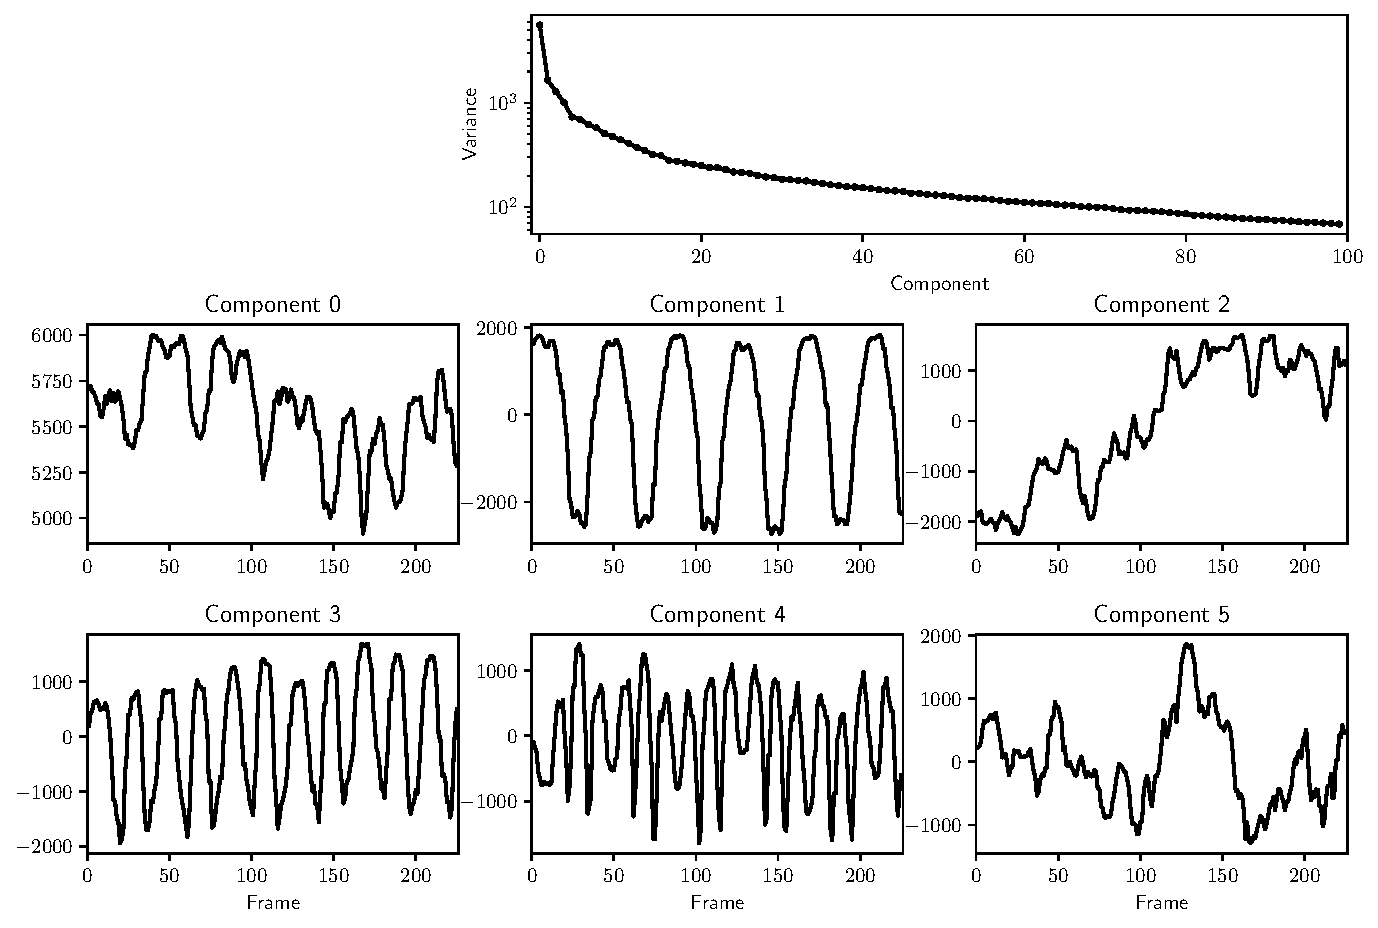
\includegraphics[width=\textwidth]{PCA_1.pdf}
        \caption{Test 1. Ideal cade. The covariance of the first 100 principal
        components along with the first 6 components. \label{fig:test_1}}
    \end{figure}

    \begin{figure}[p]
        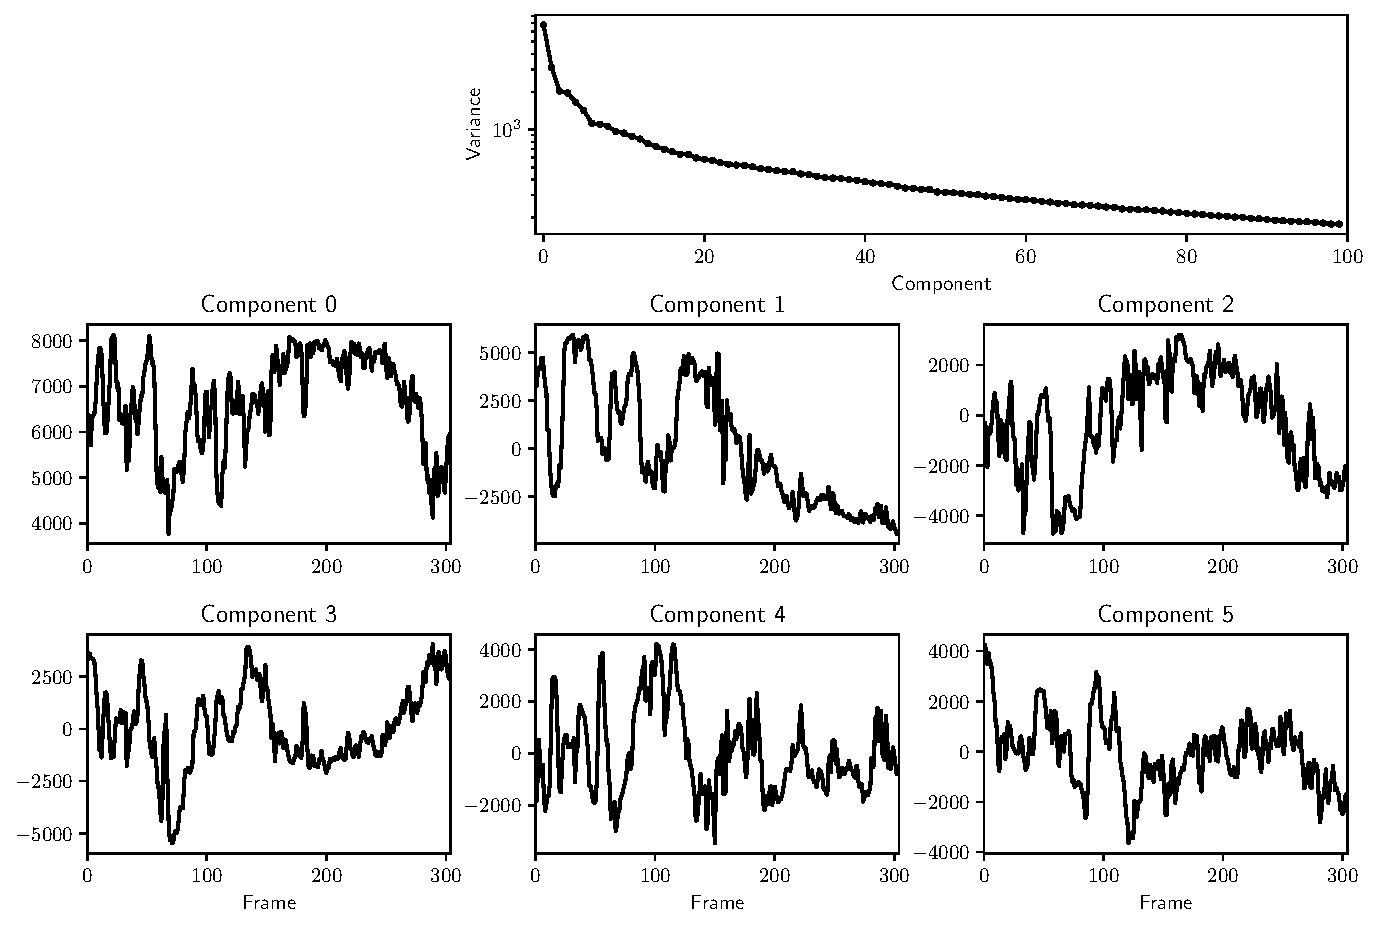
\includegraphics[width=\textwidth]{PCA_2.pdf}
        \caption{Test 2. Noisy cade. The covariance of the first 100 principal
        components along with the first 6 components. \label{fig:test_2}}
    \end{figure}

    \begin{figure}[p]
        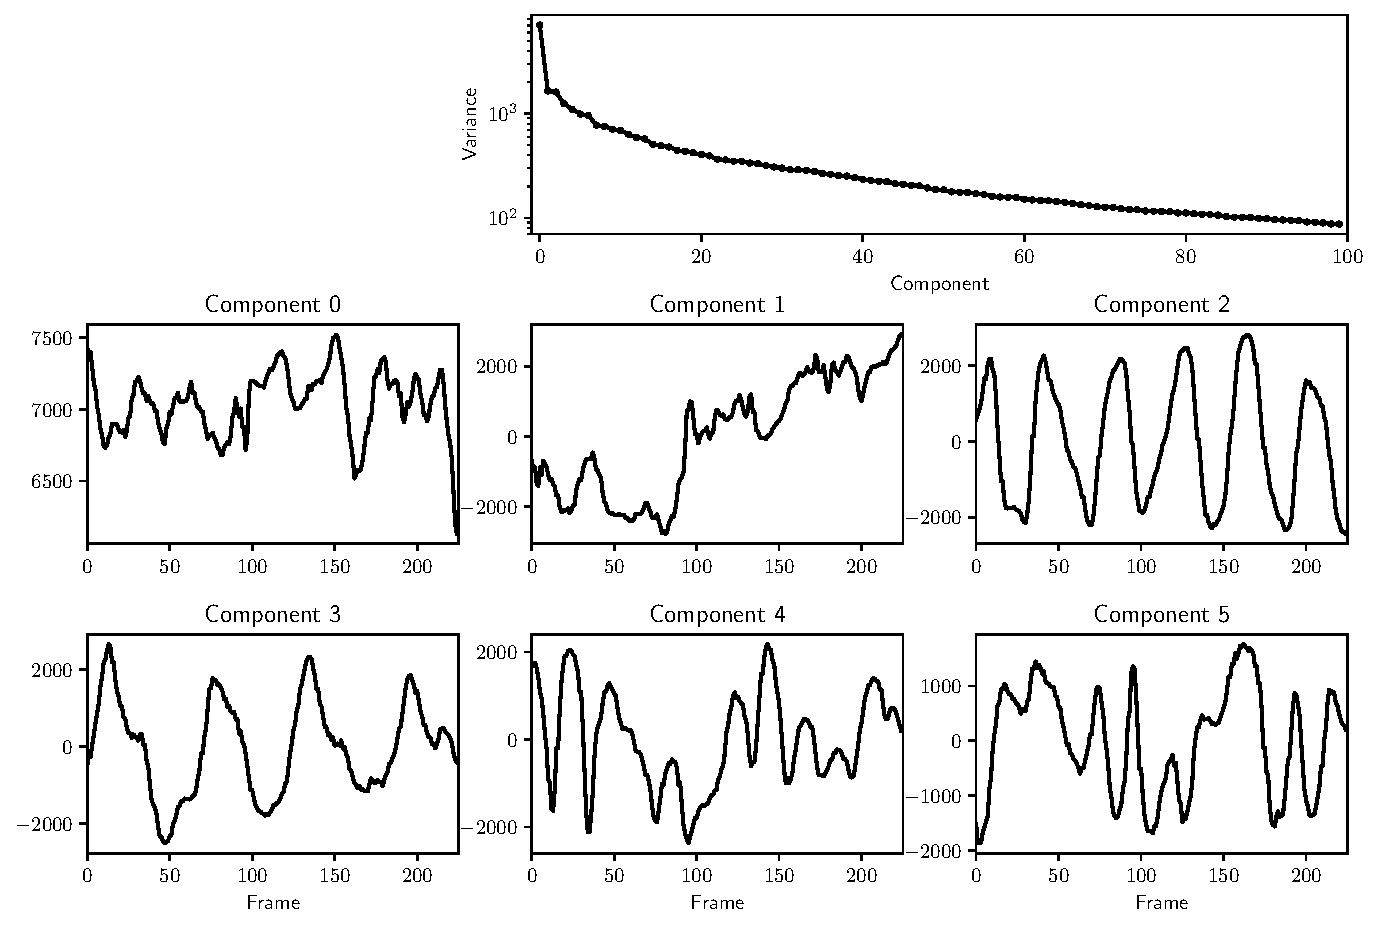
\includegraphics[width=\textwidth]{PCA_3.pdf}
        \caption{Test 3. Horizontal displacement. The covariance of the first
        100 principal components along with the first 6 components.
        \label{fig:test_3}}
    \end{figure}

    \begin{figure}[p]
        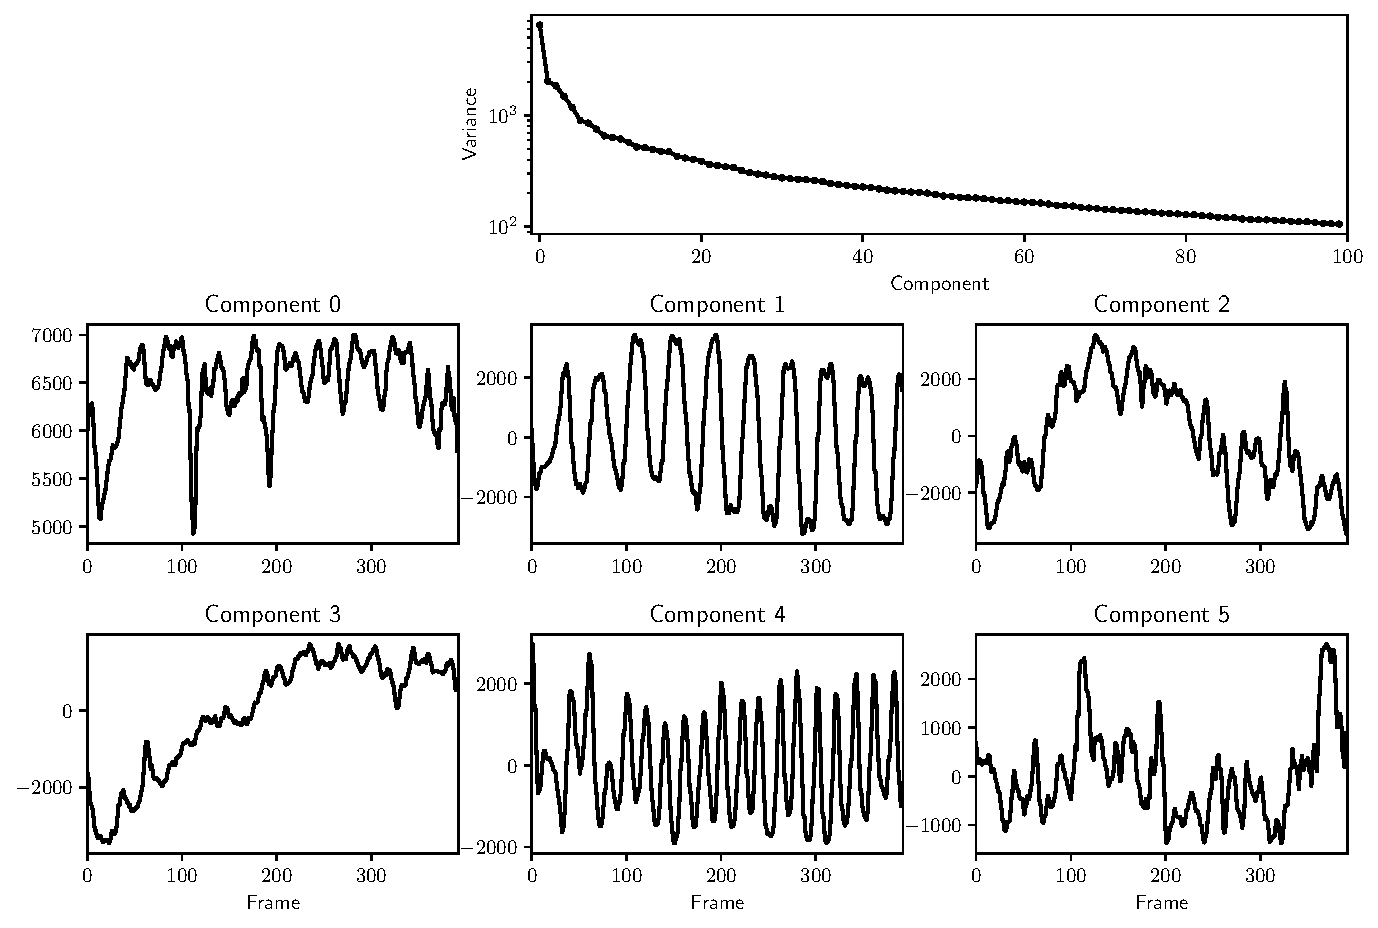
\includegraphics[width=\textwidth]{PCA_4.pdf}
        \caption{Test 4. Horizontal displacement and rotation. The covariance of
        the first 100 principal components along with the first 6 components.
        \label{fig:test_4}}
    \end{figure}


    \section{Summary and Conclusions}
    PCA was preformed on four different cases of a spring mass system recorded
    with cameras in different perspectives. The cases where the camera remains
    fixed and the mass moves without rotating have quality representation in the
    principal components. Camera shake rendered the data almost useless, as
    no part of the mass motion could be identified. Rotation of the mass
    confused the results but not so badly as to obscure all the physics.

    There are several additions that could improve the results of this
    particular problem. First, I could have used a wavelet transform to 
    identify edges or compress the data before applying PCA. Instead of using
    monochrome images, I could have used a channel that maximized the mass's
    contrast against the wall. If data could be recollected, longer videos would
    also improve identifying components of the spring mass system.

    \bibliographystyle{ieeetr}
    \bibliography{bibliography}

    \FloatBarrier
    \newpage
    \appendix
    Here is a \href{https://github.com/bagriffith/AMATH582/tree/main/HW3}
    {link to the Github repository for this project}.
    \section{Python Functions}
    % Use PyDoc to generate
    \subsection{dmd}

\subsubsection{dmd}

\begin{Shaded}
\begin{Highlighting}[]
\NormalTok{dmd(X2, u, s, vh)}
\end{Highlighting}
\end{Shaded}

Returns the DMD modes and complex frequencies for the system.

\textbf{Arguments}:

\begin{itemize}
\tightlist
\item
  \texttt{X2} \emph{array-like} - The X\_2\^{}M matrix
\item
  \texttt{u} \emph{array-like} - The U matrix of the X\_1\^{}M-1 SVD
\item
  \texttt{s} \emph{array-like} - The s array of the X\_1\^{}M-1 SVD
\item
  \texttt{vh} \emph{array-like} - The vh matrix of the X\_1\^{}M-1 SVD
\end{itemize}

\textbf{Returns}:

\begin{itemize}
\tightlist
\item
  \texttt{ndarray} - Array of complex frequencies for DMD modes
\item
  \texttt{ndarray} - Matrix with rows of the DMD modes
\end{itemize}

\subsubsection{x\_dmd}

\begin{Shaded}
\begin{Highlighting}[]
\NormalTok{x_dmd(t, psi, w, b)}
\end{Highlighting}
\end{Shaded}

The DMD approximation of x(t).

\textbf{Arguments}:

\begin{itemize}
\tightlist
\item
  \texttt{t} \emph{float} - The time in frames
\item
  \texttt{psi} \emph{array-like} - Matrix with rows of the DMD modes
\item
  \texttt{w} \emph{array-like} - Array of complex frequencies for DMD
  modes
\item
  \texttt{b} \emph{array-like} - Array of initial values of the DMD
  modes
\end{itemize}

\textbf{Returns}:

\begin{itemize}
\tightlist
\item
  \texttt{ndarray} - DMD approximation of pixels at t
\end{itemize}

\subsubsection{frame\_bg\_sep}

\begin{Shaded}
\begin{Highlighting}[]
\NormalTok{frame_bg_sep(t, X, psi, w, b)}
\end{Highlighting}
\end{Shaded}

Separate the forground and background of frame t

\textbf{Arguments}:

\begin{itemize}
\tightlist
\item
  \texttt{t} \emph{int} - The time in frames
\item
  \texttt{psi} \emph{array-like} - Matrix with rows of the DMD modes
\item
  \texttt{w} \emph{array-like} - Array of complex frequencies for DMD
  modes
\item
  \texttt{b} \emph{array-like} - Array of initial values of the DMD
  modes
\end{itemize}

\textbf{Returns}:

\begin{itemize}
\tightlist
\item
  \texttt{ndarray} - Foreground array
\item
  \texttt{ndarray} - Background array
\end{itemize}

\subsubsection{show\_frame}

\begin{Shaded}
\begin{Highlighting}[]
\NormalTok{show_frame(frame, shape, path_out)}
\end{Highlighting}
\end{Shaded}

Plot the frame provided.

\textbf{Arguments}:

\begin{itemize}
\tightlist
\item
  \texttt{frame} \emph{array-like} - 1 D array of pixels
\item
  \texttt{shape} \emph{tuple} - The shape of the image (pixels\_y,
  pixels\_x)
\item
  \texttt{path\_out} \emph{str} - Path to save figure to
\end{itemize}

\subsection{svd}

\subsubsection{plot\_n\_modes}

\begin{Shaded}
\begin{Highlighting}[]
\NormalTok{plot_n_modes(X, V, n, shape, path_out)}
\end{Highlighting}
\end{Shaded}

Shows the numbers represented with the selected number of SVD modes

\textbf{Arguments}:

\begin{itemize}
\tightlist
\item
  \texttt{X} \emph{array\_like} - Data matrix with rows of images
\item
  \texttt{V} \emph{array\_like} - Matrix with mode vectors as columns
\item
  \texttt{n} \emph{int} - Number of modes to use in the representation
\item
  \texttt{shape} \emph{tuple} - The shape of the image (pixels\_y,
  pixels\_x)
\item
  \texttt{path\_out} \emph{str} - Path to save figure to
\end{itemize}

\subsubsection{plot\_mode\_fraction}

\begin{Shaded}
\begin{Highlighting}[]
\NormalTok{plot_mode_fraction(s, path_out)}
\end{Highlighting}
\end{Shaded}

Plots the fraction of power represented with n modes

\textbf{Arguments}:

\begin{itemize}
\tightlist
\item
  \texttt{s} \emph{array-like} - 1D arrray of the variances of the
  principal components.
\item
  \texttt{path\_out} \emph{str} - Path to save figure to
\end{itemize}

\subsection{loadVid}

\subsubsection{open\_video}

\begin{Shaded}
\begin{Highlighting}[]
\NormalTok{open_video(vid_path)}
\end{Highlighting}
\end{Shaded}

Loads the video matrices

\textbf{Arguments}:

\begin{itemize}
\tightlist
\item
  \texttt{vid\_path} \emph{str} - Path to the video file
\end{itemize}

\textbf{Returns}:

\begin{itemize}
\tightlist
\item
  \texttt{ndarray} - X\_1\^{}M-1
\item
  \texttt{ndarray} - X\_2\^{}M
\end{itemize}


    \section{Python Code}
    \subsection{pca.py}
    \inputminted{python}{../code/pca.py}


\end{document}
